\chapter{多用户下的可验证对称加密搜索方案研究}
\label{cha:multi-user}
\section{引言}
本章在\single 的基础上,提出了一种适用于多用户场景的可验证对称加密搜索方案\multi 。该方案同样可以与任意多用户场景下的加密搜索方案结合,来为其提供结果验证功能。与\single 方案不同的是,在多用户的场景下,即数据共享的情况下,数据持有者与数据搜索者产生了分离。数据持有者一方面需要对数据搜索者进行访问控制,以确保数据搜索者的合法性,并且确保数据搜索者只能读取数据而无法写入数据。另一方面,为了保证数据新鲜性,数据持有者还需要在数据发生了更新时,告知数据搜索者。我们将通过公私钥机制解决访问控制问题,并通过时间戳链机制解决数据新鲜性问题。本章的主要内容安排如下:首先介绍了多用户场景下(即数据持有者和数据搜索用户分离)的系统框架,明确了该框架的参与方及所承担的计算任务;随后通过一个抽象定义对该方案工作的流程进行了说明;算法分析部分对抽象定义中的具体算法进行了详细分析;最后,通过安全性分析和实验结果验证了本方案的安全性和有效性。



\section{系统架构}

\begin{figure}[t]
\centering
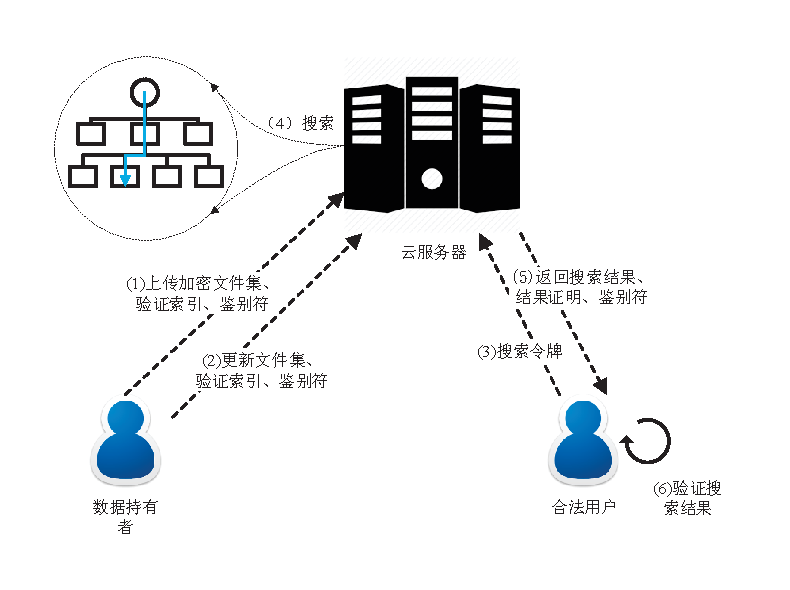
\includegraphics[width=5 in]{fig/GM-VSSE}
\DeclareGraphicsExtensions.
\caption{多用户场景下的可验证对称加密搜索框架\multi}
\label{fig:GM-VSSE}
\end{figure}

多用户场景下的可验证对称加密搜索方案\multi 如图~\ref{fig:GM-VSSE}所示,数据持有者和数据搜索用户产生了分离。首先数据持有者仍然需要对文件集进行处理,得到验证索引,同时他还需要生成一个鉴别符,将二者同时上传给云服务器。数据持有者在更新数据时,需要同时更新云端的验证索引和鉴别符。数据持有者可以将数据搜索者授权为一个合法用户。合法用户可以通过提交搜索令牌来对数据持有者的加密文件集进行搜索。云服务器在收到该搜索令牌以后,需要根据某一加密搜索方案向其返回加密搜索结果,同时返回结果证明以及鉴别符。通过这种方式,合法用户可以按需获取搜索结果并进行结果验证。


\section{方案流程}
在描述\multi 方案的工作流程前,我们先回顾多用户对称加密搜索方案的常见定义。
\begin{definition}[\textbf{MSSE 方案}]\label{def:MSSE}
  {\itshape
      一个支持文件更新的$MSSE$方案,参与方有三个, 分别为数据持有者,合法用户以及半可信的云服务器。数据持有者向云服务器提供加密数据集和搜索索引,同时数据持有者可以对合法用户进行注册和撤销。云服务器可以为合法用户提供搜索功能。一个$MSSE$方案是以下八个算法的集合:
      \begin{itemize}
        \item $KGen_{\mathcal{MSSE}}(1^k) \rightarrow \{\mathcal{K},K_O\}$: 是由数据持有者执行的秘钥生成算法。它将一个安全参数作为输入,输出一系列对称秘钥$\mathcal{K}$和一个用户私钥$K_O$。
        \item $EnrollUser_{\mathcal{MSSE}}(K_O,U) \rightarrow \{K_U\}$: 是由数据持有者执行的用户注册算法。它将数据持有者的私钥 $K_O$ 和待注册用户的身份证明 $U$作为输入,输出该用户的私钥$K_U$。数据持有者将私钥$K_U$ 发送给用户$U$。该算法将一个用户添加到了数据持有者的合法用户集合中,即授权该用户对数据持有者的数据进行搜索。
        \item $RevokeUser_{\mathcal{MSSE}}(K_O,U) \rightarrow \{b\}$: 是由数据持有者执行的用户撤销算法。它将数据持有者的私钥 $K_O$ 和待注册用户的身份证明 $U$, 输出一个比特$b$。如果$b=1$表示撤销成功,反之。该算法将一个用户从数据持有者的合法用户集中移除,即取消该用户对数据持有者云端加密数据的搜索权限。
        \item $Init_{\mathcal{MSSE}}(\mathcal{K}, \mathcal{D}) \rightarrow \{\gamma, \mathcal{C}\}$: 是由数据持有者执行的初始化算法。它将对称秘钥$\mathcal{K}$和明文文件集$\mathcal{D}$作为输入,输出搜索索引$\gamma$和密文文件集$\mathcal{C}$。数据持有者将搜索索引$\gamma$和密文文件集$\mathcal{C}$上传给云服务器。
        \item $UpdateToken_{\mathcal{MSSE}}(\mathcal{K}, d) \rightarrow \{\tau_u\}$: 是由数据持有者执行的更新令牌生成算法。它将对称秘钥$\mathcal{K}$和需要更新的文件$d$作为输入,输出一系列更新令牌$\tau_u$。数据持有者将更新令牌$\tau_u$上传给云服务器。
        \item $Update_{\mathcal{MSSE}}(\gamma, \tau_u) \rightarrow \{\gamma'\}$: 是由云服务器执行的更新算法。它将搜索索引$\gamma$和更新令牌$\tau_u$作为输入,输出更新后的搜索索引$\gamma'$。
        \item $SearchToken_{\mathcal{MSSE}}(\mathcal{K}, w) \rightarrow \{\tau_{w}\}$: 是由合法用户执行的搜索令牌生成算法。它将对称秘钥$\mathcal{K}$和某一关键字$w$作为输入,输出与该关键字相关搜索令牌$\tau_{w}$。合法用户将该搜索令牌 $\tau_{w}$上传给云服务器进行搜索。
        \item $Search_{\mathcal{MSSE}}(\gamma, \tau_{w}) \rightarrow \{C_w\}$: 是由云服务器执行的搜索算法。它将搜索索引$\gamma$和搜索令牌$\tau_{w}$作为输入,输出搜索结果$C_w$。云服务器将搜索结果$C_w$返回给合法用户。
      \end{itemize}
      }
\end{definition}

注意,这里需要说明的是,本方案的目的不是设计多用户的对称加密搜索方案,而是为这些已有的多用户加密搜索方案提供结果验证功能。本方案在\single 的基础上进行了改进,验证索引的构建仍然需要利用MPT和增量哈希技术,同时\multi 方案还使用了时间戳链和公私钥加密机制来实现跨用户的数据新鲜性和数据完整性验证。\multi 方案的具体定义如下。

\begin{definition}[\textbf{\multi 方案}]\label{def:multi}
  {\itshape
      在 \multi 方案中,参与方有三个, 分别为数据持有者,合法用户以及不可信的云服务器。数据持有者向云服务器提供一个验证索引和鉴别符,使得云服务器可以为合法用户提供搜索结果证明,来确保加密搜索结果的新鲜性和完整性。一个\multi 方案是以下八个算法的集合:
      \begin{itemize}
        \item $KGen(1^k) \rightarrow \{K_1,K_2,K_3,K_O, (ssk, spk)\}$: 是由数据持有者执行的秘钥生成算法。它将一个安全参数作为输入,输出对称秘钥 $K_1,K_2,K_3$ ,数据持有者私钥$K_O$和一对签名公私钥对 $(ssk, spk)$。
        \item $EnrollUser(K_O,U) \rightarrow \{K_U\}$: 是由数据持有者执行的用户注册算法。它将数据持有者的私钥 $K_O$ 和待注册用户的身份证明 $U$作为输入,输出该用户的私钥$K_U$。数据持有者将私钥$K_U$以及对称秘钥$K_1,K_2,K_3$和签名公钥$spk$发送给用户$U$。该算法将一个用户添加到了数据持有者的合法用户集合中,即授权该用户对数据持有者的数据进行搜索。
        \item $RevokeUser(K_O,U) \rightarrow \{b\}$: 是由数据持有者执行的用户撤销算法。它将数据持有者的私钥 $K_O$ 和待注册用户的身份证明 $U$, 输出一个比特$b$。如果$b=1$表示撤销成功,反之。该算法将一个用户从数据持有者的合法用户集中移除,即取消该用户对数据持有者云端加密数据的搜索权限。

        \item $Init(K_1,K_2,K_3, ssk, \mathcal{D}) \rightarrow \{\lambda,\pi\}$: 是由数据持有者执行的初始化算法。它将对称秘钥 $K_1,K_2,K_3$,签名私钥 $ssk$ 和明文文件集 $\mathcal{D}$ 作为输入,输出验证索引 $\lambda$ 和鉴别符 $\pi$。数据持有者在本地保存验证索引$\lambda$的根节点哈希$rt$,并将验证索引$\lambda$和鉴别符 $\pi$上传给云服务器。
        \item $UpdateToken(K_1,K_2,K_3, ssk, d) \rightarrow \{\tau_u, \pi\}$: 是由数据持有者执行的更新令牌生成算法。它将对称秘钥$K_1,K_2,K_3$,签名私钥$ssk$和需要更新的文件$d$作为输入,输出一系列更新令牌$\tau_u$和鉴别符 $\pi$。数据持有者将更新令牌$\tau_u$和鉴别符$\pi$上传给云服务器。
        \item $Update(\lambda, \tau_u) \rightarrow \{\lambda',\rho_u\}$: 是由云服务器执行的更新算法。它将验证索引$\lambda$和更新令牌$\tau_u$作为输入,输出更新后的验证索引$\lambda'$和更新证明$\rho_u$。云服务器将更新证明$\rho_u$返回给数据持有者。
        \item $VerifyUpdate(rt,\tau_u,\rho_u) \rightarrow \{rt'\}$:是由数据持有者执行的更新算法。它将验证索引的根哈希 $rt$,更新令牌$\tau_u$和服务器返回的更新证明 $\rho_u$ 作为输入,输出新的根哈希$rt'$。若更新证明$\rho_u$验证通过,则输出更新后的根哈希$rt'$,若更新证明验证失败,则输出的根哈希$rt'$与原始根哈希$rt$相同。
        \item $SearchToken(K_1, w) \rightarrow \{\tau_{w}\}$: 是由合法用户执行的搜索令牌生成算法。它将对称秘钥$K_1$和某一关键字$w$作为输入,输出与该关键字相关搜索令牌$\tau_{w}$。合法用户将该搜索令牌 $\tau_{w}$上传给云服务器进行搜索。
        \item $Prove(\lambda, \tau_{w}, t_q) \rightarrow \{\rho,\pi^t_q, \pi_c\}$:是由云服务器执行的结果证明生成算法。它将验证索引$\lambda$,搜索令牌$\tau_{w}$以及合法用户提交查询的时间$t_q$作为输入,输出$\rho$和两个鉴别符$\pi^t_q$,$\pi_c$作为结果证明。云服务器将结果证明$\rho$,$\pi^t_q$,$\pi_c$返回给合法用户。
        \item $Verify(K_1,K_2,K_3, spk, C_w, \rho_s, \pi^t_q, \pi_c, \tau_{w},rt) \rightarrow \{b\}$: 是由合法用户执行的验证算法。它将对称秘钥$K_1,K_2,K_3$,签名公钥$spk$,加密搜索结果$C_w$,结果证明$\rho_s$,鉴别符$\pi^t_q$, $\pi_c$,搜索令牌$\tau_{w}$和保留的验证索引根哈希$rt$作为输入,输出一个比特$b$,代表接受或者拒绝该搜索结果。其中,该算法包括了两个子算法,分别为 $Check$ 算法和 $Generate$ 算法,它们分别可以定义为 $Check(K_3, spk, \pi^t_q, \pi_c) \rightarrow \{b\}$ 和 $Generate(K_1,K_2,K_3,C_w,\rho,\tau_{w},\pi^t_q) \rightarrow \{b\}$.
      \end{itemize}
      }
\end{definition}

\section{具体方案}
本节中,我们将阐述\multi 方案,即多用户场景下的可验证加密搜索方案。注意,由于数据在多个用户之间共享,当数据持有者的数据需要更新时,如何将更新信息同步给多个用户,从而确保数据的新鲜性是本方案的重要挑战。一个简单的想法是,由于验证索引的根哈希是数据新鲜性和数据完整性的保证,在数据持有者需要更新数据时,他只需将更新后的验证索引根哈希值发送给所有的合法用户即可。但这种方式在数据需要频繁更新的场景下,势必给数据持有者带来巨大的通信开销。并且,这种推送的方法存在带宽浪费,即某些合法用户搜索数据的频率可能较低,在两次推送时间间隔内,并没有数据搜索需求。考虑到该问题,我们提出了一种由合法用户按需获取验证索引根哈希的方式。该方法引入了由时间戳链构造的鉴别符,将验证索引的根哈希值与时间戳绑定,使得用户在搜索数据时,能够获取到最新的根哈希值,用以对数据的新鲜性进行验证。本节的内容安排如下,首先我们将描述如何建立和更新鉴别符,然后我们给出了通过鉴别符验证数据新鲜性的方法,最后通过一个简单的例子介绍了本方案的工作细节。

\subsection{构建及更新时间戳链}
由于云服务器不可信,当数据持有者向云服务器发送了多个鉴别符以后,云服务器有可能会向合法用户重放之前收到的鉴别符,以此来破坏数据新鲜性。针对该问题,本方案采用了时间戳链机制来构造鉴别符,而不仅仅是将验证索引根哈希与时间戳绑定。它使得合法用户可以通过该时间戳链来追踪其中包含的鉴别符,从而确保自身拿到的根哈希值为最新的数据。注意,我们采用的时间戳链方案与可验证对称加密搜索方案~\cite{stefanov2014practical}不同。他们的方案仅仅能在单用户的场景下工作,即在用户持有更新信息的场景下工作。因此,他们的方案不能用户多用户场景下的数据新鲜性验证。



在方案开始工作前,我们先对方案的设定进行描述,首先数据持有者需要为鉴别符设定一个更新周期 (Update Interval)\footnote{在实验验证环节,我们将展示更新周期与结果验证时延的相关性~\ref{sec:experiments}},即设置固定更新时间点为$\{up_1, up_2, \cdots, up_i, \cdots, up_m\}$。如果更新周期内数据持有者的数据产生了更新,则数据持有者需要生成鉴别符进行上传,否则,数据持有者只需要在固定更新时间点对鉴别符进行上传。注意,更新周期可以由数据持有者根据其更新频率来控制。 一般来说,如果数据持有者的更新频率较高,则更新周期可以设置短一些,以保证一个更新周期内的鉴别符不会过长,并且验证的时延也会减少。但这会给数据持有者带来相对较高的更新负载。在我们的实验部分\ref{sec:experiments},我们将会展示用户验证时延和数据持有者带宽开销之间的关系。
这里我们将使用网络时间协议 (Network Time Protocol, NTP)~\cite{mills1991internet, mills2010network}来对云服务器,数据持有者以及合法用户进行时间同步。注意,时钟同步的精确度目前已经可以达到几毫秒甚至是几十微秒~\cite{kopetz1987clock, elson2002fine, zhou2007accurate},足以保证\multi 方案的验证正确性。此外,一个恶意的云服务器有可能会伪造时钟信息,但他永远无法伪造时间戳链信息,因为时间戳链的信息由数据持有者的签名私钥进行了保证。接下来我们将阐释方案细节。


首先,我们将阐述数据持有者如何通过时间戳链构造鉴别符。
为了防止云服务器重放鉴别符,我们设计了一种基于时间戳链的机制来检测云服务器的恶意行为。我们通过将旧的鉴别符嵌套进新的鉴别符的方式,使得鉴别符串联起来形成链。如公式\ref{equ:timestamp-chain}所示,我们将旧的鉴别符$\pi$与时间戳$tp$和验证索引的根哈希$rt$进行连接,并将联合后的三者用对称秘钥$K_3$加密,同时使用数据持有者的签名私钥$ssk$进行签名,从而生成新的鉴别符。如果验证索引在一个更新周期内没有更新,则数据持有者只需要在下一个固定更新时间点对鉴别符中的时间戳进行更新。如果数据持有者的文件集在更新周期内产生了更新,即验证索引的根哈希产生了更新,则数据持有者需要用更新后的根哈希和最新的时间戳来构建一个新的鉴别符,并上传给云服务器。注意,在每一个更新周期内会形成一个时间戳链,每个时间戳链在下一个更新周期开始时结束,即每个时间戳链中的最后一个鉴别符是在下一个固定更新时间点生成的。换句话说,每一个更新周期内的鉴别符是连接在一起的,而不同更新周期内的鉴别符是不相关的。


\begin{equation}
  \label{equ:timestamp-chain}
    \left\{
    \begin{array}{ll} % \begin{eqnarray}好像也可以。
      \pi_{i, 0} = (\alpha_{i, 0}, \mathsf{Sig}_{ssk}(\alpha_{i, 0})),~~~~~~~~~~~up_i < tp_{i, 0} \leq up_{i+1} \\
      \alpha_{i, 0} = Enc_{K_3}(rt_{i, 0}||tp_{i, 0}) \\
      \cdots \\

     \pi_{i, j} = (\alpha_{i, j}, \mathsf{Sig}_{ssk}(\alpha_{i, j})),~~~~~~~~~~~tp_{i, j-1} < tp_{i, j} \leq up_{i+1}  \\
     \alpha_{i, j} = Enc_{K_3}(rt_{i, j}||tp_{i, j}||\alpha_{i, j-1}) \\
      \cdots  \\
     \pi_{i, n} = (\alpha_{i, n}, \mathsf{Sig}_{ssk}(\alpha_{i, n})),~~~~~~~~~~~tp_{i, n}=up_{i+1} \\
     \alpha_{i, n} = Enc_{K_3}(rt_{i, n}||tp_{i, n}||\alpha_{i, n-1})
    \end{array}
    \right.
  \end{equation}

\noindent 这里 $i$ 代表第 $i$个更新周期, $j$ 代表该更新周期内的第 $j$个鉴别符.

在这种设置下,当一个合法用户发起了一次搜索时,云服务器需要将最新的鉴别符发送给用户。用户可以通过解密鉴别符从其中得到验证索引的根哈希值$rt$和时间戳$tp$。如果时间戳$tp$在最近一次固定更新时间点之前,则可以认为服务器发回了旧的鉴别符,产生了恶意行为。这种方式保证了云服务器无法在当前更新周期外产生数据新鲜性攻击。

然而,如果云服务器只传送最新的鉴别符给用户,它仍然可以在当前更新周期内产生数据新鲜性攻击。具体而言,如果在当前更新周期内,数据持有者的文件集产生了一次或者多次的更新,即数据持有者在该更新周期内,上传了多个鉴别符,则云服务器可以发送该更新周期内的任意一个旧的鉴别符来发起数据新鲜性攻击。

当然,如果用户对数据新鲜性的要求不高,那么数据新鲜性的验证到此即可。但对于某些必须保证数据实时同步的用户,我们还需要解决当前更新周期内发生数据新鲜性攻击的问题。为了解决该问题,云服务器除了需要将搜索时刻的鉴别符发送给用户以外,还需要将当前时间戳链中的最后一个鉴别符发送给用户。我们将当前更新周期内时间戳链的结束时间点成为检测点(checkpoint)。通过这种方式,用户可以解密在检测点收到的鉴别符,并使用该鉴别符追踪在搜索时刻收到的鉴别符,以此来判定搜索时刻收到的鉴别符是否为搜索时刻最新的鉴别符,从而防止了云服务器在当前更新周期内发起数据新鲜性攻击。在下一小节,我们将详细描述用户如何通过两个鉴别符检测云服务器是否发起了数据新鲜性攻击。


\subsection{结果验证}

\begin{algorithm}[t]
  \caption{$Check$算法}
  %\setcounter{algorithm}{2.1}
  \label{alg:check}
  \begin{algorithmic}[1]
    \REQUIRE {$K_3$: 对称秘钥; $spk$: 验证签名的公钥; $\pi^t_q$: 在搜索时刻 $t$返回给数据搜索用户的鉴别符; $\pi_c$: 在检测点返回给用户的鉴别符。}
    \ENSURE {$b \in \{0,1\}$, 如果 $b=1$, $Check$算法成功,否则失败。}
              \STATE{令 $\pi^t_q = \{\alpha^t_q, Sig^t_q\}$, $\pi_c = \{\alpha_c, Sig_c\}$}
              \IF{$\alpha^t_q \neq (Sig^t_q)_{spk}$ $\vert \vert$ $\alpha_c \neq (Sig_c)_{spk}$}
                \RETURN{$b = 0$}
              \ENDIF
              \STATE {$(rt^t_q, tp^t_q, \alpha) \leftarrow Dec_{K_3}(\alpha^t_q)$}
              \IF{$tp^t_q$ 早于最近一个更新时间点}
                \RETURN {$b = 0$}
              \ENDIF
              \STATE {令 $\alpha_k = \alpha_c$}
              \FOR {$\alpha_k \neq \emptyset$}
                    \STATE {$(rt_k, tp_k, \alpha_{k-1}) \leftarrow Dec_{K_3}(\alpha_k)$}
                    \IF {$tp_k < t$}
                      \STATE{break}
                    \ENDIF
                    \STATE {令 $\alpha_k = \alpha_{k-1}$}
              \ENDFOR
              \IF {$\alpha_k = \alpha^t_q ||\alpha_k = \emptyset$}
                  \RETURN {$b = 1$}
              \ELSE
                  \RETURN {$b = 0$}
              \ENDIF
  \end{algorithmic}
\end{algorithm}

\begin{algorithm}[t]
  \caption{Verify算法}
  \label{alg:verify2}
  \begin{algorithmic}[1]
    \REQUIRE {$K_1,K_2,K_3$: 对称秘钥;$spk$: 签名所使用的公钥; $C_{w}$: 加密搜索结果;$\rho_s$: 加密搜索结果证明;$\tau_{w}$: 搜索令牌;$\pi^t_q$: 在搜索时刻 $t$ 收到的鉴别符;$\pi_c$: 在检测点收到的鉴别符;}
    \ENSURE {$b \in \{0,1\}$, 如果 $b = 1$, 接受该结果;否则拒绝该结果。}
          \STATE {$b \leftarrow Check (K_3,spk, \pi^t_q, \pi_c)$}
          %\IF{$b_1=1$}K_1,K_2,K_3,C_w,\rho,\tau_{w},\pi^t_q
          \RETURN {$b \leftarrow b\quad  \&\&\quad Generate(K_1,K_2,K_3,C_w,\rho,\tau_{w},\pi^t_q)$}

          %\ELSE
          %  \RETURN {$reject$}
          %\ENDIF
  \end{algorithmic}
\end{algorithm}

\multi 方案中,数据持有者的验证算法$Verify$可以拆分为两个子算法$Check$和$Generate$,其中$Check$算法主要用于对鉴别符的验证,保证鉴别符的最新就保证了用户收到的验证索引根哈希为最新,从而防止了数据新鲜性攻击。$Generate$算法在$Check$算法后执行,它通过加密搜索结果,搜索令牌,结果证明和$Check$算法解密得到的最新根哈希可以完成对数据完整性的验证。该算法的具体流程与\single 方案中的$Verify$算法相同,只是$Generate$算法在与重构出的根哈希进行对比时,使用的根哈希为从鉴别符中解密得到的根哈希,而不是自身保留的根哈希,因此,这里不再赘述。

算法~\ref{alg:check}展示了$Check$算法的伪代码,该算法由合法用户执行,用以确保鉴别符没有被重放。
假设$\pi^t_q$为用户在搜索时刻$t$收到的鉴别符, $\pi_c$为用户在检测点收到的鉴别符。首先我们需要通过签名公钥$spk$确保两个鉴别符都来自于数据持有者。接着,我们需要通过鉴别符$\pi^t_q$中的$\alpha^t_q$来确保该鉴别符的时间戳不会早于该更新周期。随后,我们需要通过$\pi_c$中的$\alpha_c$不断解密得到$rt_k||tp_k||\alpha_{k-1}$,直到我们找到某个时间戳$tp_k < t$,或者找到$\alpha_k = \emptyset$。我们将  $\alpha_k$与$\alpha^t_q$和$\emptyset$进行对比。如果$\alpha_k$与两者均不相等,则证明产生了数据新鲜性攻击。否则,$\alpha^t_q$就被认为是正确的,即其中包含的根哈希可以用作数据新鲜性和数据完整性的见证。



在合法用户完成了鉴别符的验证以后,即验证了数据新鲜性后,用户即可使用鉴别符$\pi^t_q$中的根哈希来对数据完整性进行验证。如算法~\ref{alg:verify2}所示,合法用户需要通过$Check$算法确保鉴别符$\pi^t_q$的正确性,从而确保其中包含的根哈希的新鲜性。如果鉴别符$\pi^t_q$验证通过,则再通过$Generate$算法比较从鉴别符$\pi^t_q$中得到的根哈希与通过搜索结果和结果证明恢复出来的根哈希是否相等。只有这两个算法都验证通过,即都输出$b=1$,$Verify$算法才验证通过,表示接受服务器返回的加密搜索结果。


%However, if the update is not frequent, the update interval can be set longer to reduce the bandwidth consumption introduced by the fixed update.
% incurred by the fixed update point.

\subsection{实例分析}

\begin{figure}[htb]
  \centering
  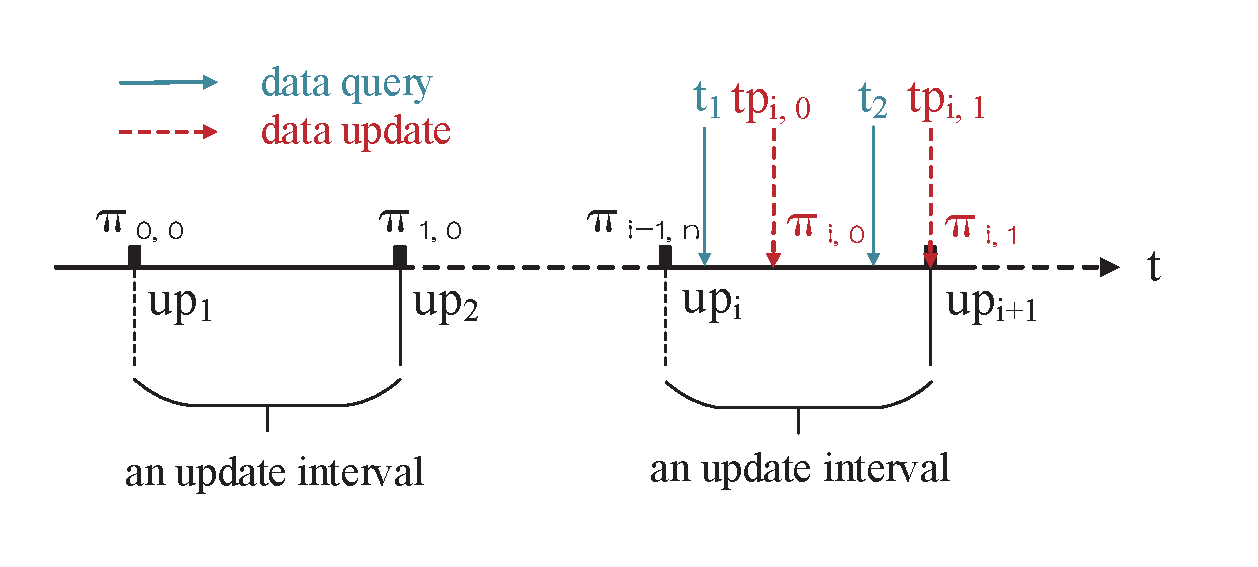
\includegraphics[width=5 in]{fig/timestamp}
  \DeclareGraphicsExtensions.
  \caption{时间戳链的简单示例}
  \label{fig:timestamp}
\end{figure}

如图~\ref{fig:timestamp}所示,横向为时间轴,红色的线表示的是数据持有者的更新时间点,蓝色的线表示的是合法用户的查询点。$(up_1,up_2,\cdots,up_i,up_{i+1})$是更新时间点,其中$(up_i,up_{i+1}]$即为一个更新周期,$up_{i+1}$为该更新周期的检测点。
每一个周期中,鉴别符都链式相连,例如图中的$\pi_{i, 0}, \pi_{i, 1}$,但是不同的更新周期内的鉴别符不相连。

让我们考虑如下几种合法用户在不同时刻发起请求的情况:(i) 第一种情况,合法用户在$t_1$时刻发起搜索请求,其中$t_1 < tp_{i, 0}$;(ii) 第二种情况,合法用户在$t_2$时刻发起搜索请求,该请求发生在一次数据更新时刻$tp_{i, 0}$之后,且云服务器发送给用户的鉴别符为$\pi_{i, 0}$;(iii)第三种情况,合法用户仍然在$t_2$时刻发起搜索请求,但是云服务器发送给用户的鉴别符为$\pi_{i-1, n}$。在最后一种情况中,一个数据新鲜性攻击产生,但是它会在检测点$up_{i+1}$被用户发现。用户将在检测点收到鉴别符$\pi_{i, 1}$,通过它用户可以验证用户在查询时刻收到的鉴别符是否正确。

我们仍然采用上述三种情况来描述合法用户验证鉴别符的过程。在上述第一种情况中,用户将收到鉴别符$\pi_{i-1, n}$ 和 $\pi_{i, 1}$,通过它们,用户可以提取出 $\alpha_{i-1,n}$ 和 $\alpha_{i,1}$,$\alpha_{i,0}$。通过$Check$算法,我们可以发现在解密了$\alpha_{i, 0}$后,得到的$\alpha$为$\emptyset$,因此$Check$算法将输出$b=1$, 表示在搜索时刻收到的鉴别符$\pi_{i-1, n}$是正确的。在第二种情况中,$\alpha_{i, 0}$ 同样通过 $\alpha_{i, 1}$ 被解密出,并且 $\alpha_{i, 0}$的时间戳已经早于 $t_2$. 我们可以通过对比发现,通过检测点收到的鉴别符$\pi_{i, 1}$循环解密出来的$\alpha_{i, 0}$ 与在搜索时刻收到的鉴别符$\pi_{i, 0}$解密出来的 $\alpha_{i,0}$ 相等。 因此 $\alpha_{i,0}$ 也被认为是正确的,即认为用户在搜索时刻收到的根哈希是正确的。然而,在最后一种情况中,我们将会发现数据新鲜性攻击,因为解密得到的$\alpha_{i, 0}$与用户在搜索时刻得到的$\alpha_{i-1, n}$不相等。

\section{安全性分析}
在本节中,我们将对\multi 方案的安全性进行证明。与\single 方案相同,我们需要从机密性和可验证性两个角度对\multi 方案进行证明。
在证明开始前,我们需要明确\multi 方案与\single 方案的差别。\multi 方案通过引入鉴别符$\pi$的方式将根哈希和时间戳进行了绑定,搜索用户通过解密鉴别符,可以得到其中包含的最新根哈希,我们通过根哈希来对数据新鲜性和数据完整性进行验证。除此之外,\multi 方案的其他步骤均与\single 方案相同。因此我们只需证明鉴别符$\pi$的引入没有破坏数据的机密性和结果的可验证性即可。我们有以下的定理:
\begin{theorem}
    如果$(ssk,spk)$是签名公私钥对,$K_3$是对称秘钥,那么\multi 方案就是机密且可验证的。
\end{theorem}

\begin{proof}
    首先证明机密性。由于鉴别符$\pi$通过数据持有者的对称秘钥$K_3$进行了加密,因此敌手只要没有该对称秘钥,即无法获知鉴别符的内容。因此鉴别符的机密性是可以保证的,即\multi 方案是机密的。
    其次证明可验证性。由于鉴别符$\pi$通过数据持有者的签名私钥$ssk$进行了签名,并且采用了对称秘钥$K_3$进行了加密。敌手没有签名私钥$ssk$和对称秘钥$K_3$就无法伪造鉴别符。因此也无法生成让合法用户验证通过的鉴别符,因此\multi 方案是可验证的。
\end{proof}

\section{实验结果}
\subsection{实验设置}
为了证明\multi 方案的有效性,我们在一台处理器为Inter Core i5 2.5GHz,内存为4G的笔记本上进行了实验,实验采用单线程执行。这里,我们的签名秘钥对采用了RSA签名,与\single 方案相同,我们同样使用了Crypto++ 5.6.5 库来实现对称加密算法。实验的数据为十次实验的平均值。
下文中,我们首先对\multi 方案引入的数据持有者端的带宽开销进行了验证,随后对\multi 方案所需的结果验证时间进行了评估。
\subsection{实验结果}
\label{sec:experiments}

图~\ref{fig:bandwidth}和图~\ref{fig:verify-2}评估了\multi 方案的开销,包括数据持有者的通信开销和合法用户的验证开销。图中的$\eta$表示数据持有者的数据更新频率。
%To evaluate the relationship between the bandwidth of the authenticator and the update interval on the data owner, we first give the formula of the bandwidth cost introduced by the authenticator as follows: $$bandwidth=\frac{\eta^2b}{2}\times \alpha + \frac{b}{\alpha}+\frac{3\eta b}{2}$$
%where $b$ is the length of the concatenation $rt||tp$. The bandwidth of the authenticator includes two part: the overhead introduced by the fixed update point and the overhead introduced by the data update.
%We present the bandwidth cost of the update frequency $\eta$ at different values as shown in
\begin{figure}[h]
\centering
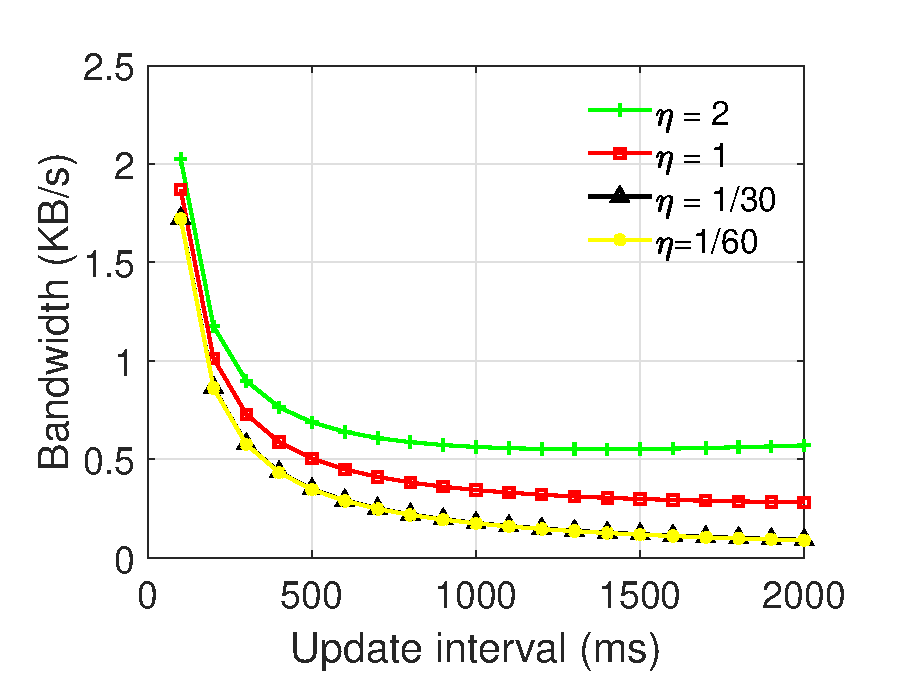
\includegraphics[width=3.5 in]{expr/bandwidth}
\DeclareGraphicsExtensions.
\caption{带宽开销}
\label{fig:bandwidth}
\end{figure}
首先,我们考虑数据持有者端的通信开销。如图~\ref{fig:bandwidth}所示,我们主要考虑由鉴别符带来的开销。这里,每一个更新周期内的第一个鉴别符大小约为176字节,包括了32字节的验证索引根哈希开销,8字节的时间戳开销,8字节的AES-CBC扩展开销,以及128字节的RSA签名开销。总体来说,鉴别符引起的带宽开销包括以下两个部分:由固定更新点导致的鉴别符更新开销和数据更新导致的鉴别符更新开销。
图~\ref{fig:bandwidth}中的曲线充分体现了这两种更新带来的开销。我们可以发现当更新周期接近0时,鉴别符到来的带宽开销接近每秒2KB,这是由固定更新点导致的鉴别符开销,因为数据持有者需要在每一个固定更新点到来时,选取当前的时间戳来重新构建鉴别符并上传。它是与带宽开销成反比的,即更新周期越小,固定更新点越密集,带宽开销越大。此外,带宽开销又随着更新周期的增长缓慢上升,这是由鉴别符自身长度增长带来的带宽开销增长。因为在数据持有者的更新频率一定的情况下,更新周期越长,一个更新周期内产生的数据更新次数将会更多。而每一次数据更新都会导致验证索引根哈希的变化,因此数据持有者需要重新选取时间戳来对更新后的根哈希进行加密上传,而一个更新周期内的鉴别符都是以链式生成的。因此更新周期越长,该更新周期内生成的鉴别符的数量也会越多,而鉴别符的长度也随着时间戳链的增长而逐渐变大。

\begin{figure}[h]
\centering
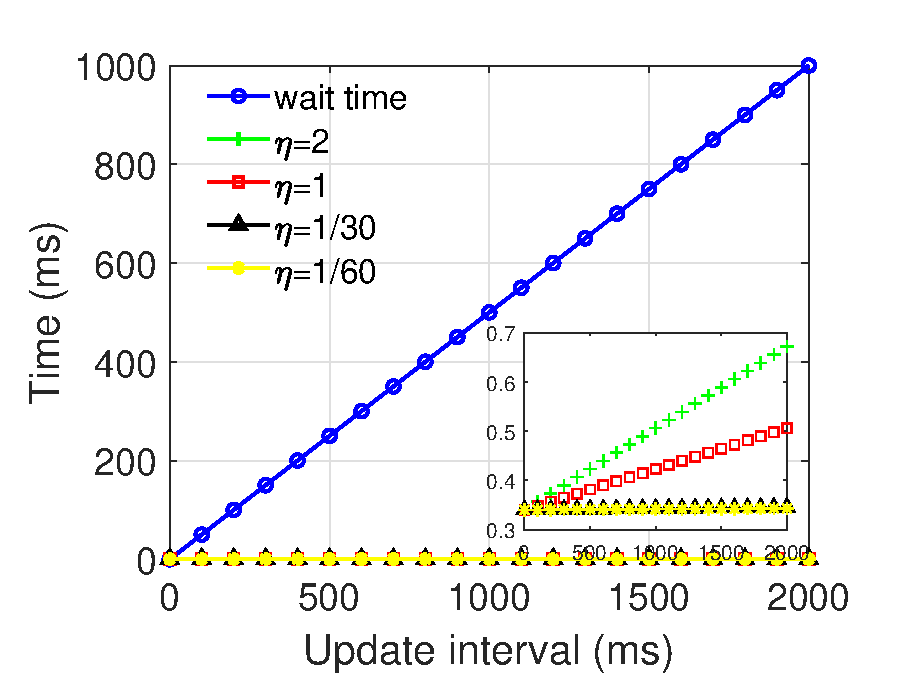
\includegraphics[width=3.5 in]{expr/verify-2}
\DeclareGraphicsExtensions.
\caption{总验证时间开销}
\label{fig:verify-2}
\end{figure}
其次,我们考虑合法用户端的验证开销。这部分开销包括用户等待检测点的时间 (wait time) 以及执行$Check$算法和$Generate$算法的时间,即$Verify$算法的时间。根据实验测量,$Generate$算法的开销为0.1毫秒,几乎可以忽略。因此图~\ref{fig:verify-2}中并未标注该部分开销。
这里, $\eta$表示数据持有者的更新频率,我们假设合法用户在一个更新周期内发起搜索请求的时刻是均匀分布的,则该用户等待检测点的时间也呈均匀分布。即等待检测点的平均时间为半个更新周期的长度,这将占整个验证时延的大部分。$Check$算法的开销与更新周期成正比,这主要由验证鉴别符的签名和解密鉴别符这两种开销导致,但是它相对等待检测点的时间是可以忽略的。需要特别说明的是,在以上的实验中,我们没有将网络的传输时间考虑在内,因为网络传输时间在不同的环境中差异非常大,并且根据我们的方案,传输时延对方案的影响不会很大。
从图\ref{fig:bandwidth}中我们可以看到,当更新频率在2Hz到1/60Hz不等时,即数据持有者的更新频率在每秒钟两次至每一分钟一次时,合法用户端的验证开销主要取决于等待检测点所需的时间,即和更新间隔的设置有关,而$Check$算法的开销几乎可以忽略不计。

综合以上的实验结果,\multi 方案引入的带宽开销和验证时延都是可以接受的。总体来说,为了在验证时延和带宽开销之间寻找一个平衡点,我们建议可以将更新周期设置在500毫秒置1500毫秒之间。在该更新周期下,数据持有者的平均带宽开销在1KB以内,而合法用户的验证时延也在200ms和800ms之间,总体来说都是可以接受的。

\section{本章总结}
本章通过方案定义,方案描述,安全性分析和实验分析等方面对\multi 方案进行了分析与阐述,\multi 方案基于不可信云存储环境,为用户提供了一种数据共享场景下的可验证对称加密搜索解决方案,总体来说,\multi 方案的贡献有以下几点:
\begin{itemize}
  \item 功能完善。\multi 方案提供了一种多用户场景下的可验证对称加密搜索方案,该方案支持在单方写/多方读的场景下工作,为数据共享场景下的可验证加密搜索提出了解决方案,使得可验证加密搜索方案的功能性更加完善。
  \item 通用性。\multi 方案可以为实现了多用户场景的对称加密搜索方案提供结果验证功能,同时确保数据新鲜性和数据完整性,使其通用性得到了进一步提升。
  \item 高效性。通过实验验证,\multi 方案为数据持有者和合法用户带来的通信开销和计算开销都很小,在方案有效的前提下保证了其高效性。
\end{itemize}
